% Chapter 4
\chapter{ارزیابی نتایج و تحلیل}
\section{معیارهای ارزیابی}
\begin{itemize}
    \item \textbf{دقت (Accuracy)}: نسبت پیش‌بینی‌های صحیح
    \item \textbf{Recall}: توانایی تشخیص نمونه‌های مثبت واقعی
    \item \textbf{AUC-ROC}: عملکرد کلی در تمام آستانه‌های طبقه‌بندی
    \item \textbf{F1-Score}: میانگین هماهنگ دقت و Recall
\end{itemize}

\section{نتایج کمی}
\begin{table}[h]
    \centering
    \begin{tabular}{|l|c|c|c|c|}
        \hline
        \textbf{مدل} & \textbf{دقت} & \textbf{Recall} & \textbf{F1} & \textbf{AUC} \\ \hline
        رندوم فارست & ۰.۹۲ & ۰.۹۵ & ۰.۸۹ & ۰.۹۸ \\ \hline
        XGBoost & ۰.۹۱ & ۰.۹۳ & ۰.۸۸ & ۰.۹۷ \\ \hline
        MLP & ۰.۸۹ & ۰.۸۵ & ۰.۸۵ & ۰.۹۵ \\ \hline
    \end{tabular}
    \caption{نتایج کمی مدل‌ها در مجموعه آزمون}
    \label{tab:results}
\end{table}

\begin{table}
    \centering
    \caption{دقت روش‌های مختلف در پژوهش \lr{RDPM}}
    \label{tab:rdpm_results}
    \begin{tabular}{@{}lccccccccc@{}}
        \textbf{تکنیک} & \textbf{Decision Tree} & \textbf{Tree Ensemble} & \textbf{Random Forest} & \textbf{Naive Bayes} & \textbf{XGBoost} & \textbf{GBT} & \textbf{SVM} & \textbf{Neural Net} \\
        \textbf{دقت (\%)} & 93.62 & 95.74 & 95.21 & 81.38 & \textbf{96.28} & 94.68 & 85.64 & 93.62 \\
    \end{tabular}
\end{table}

\begin{figure}
    \centering
    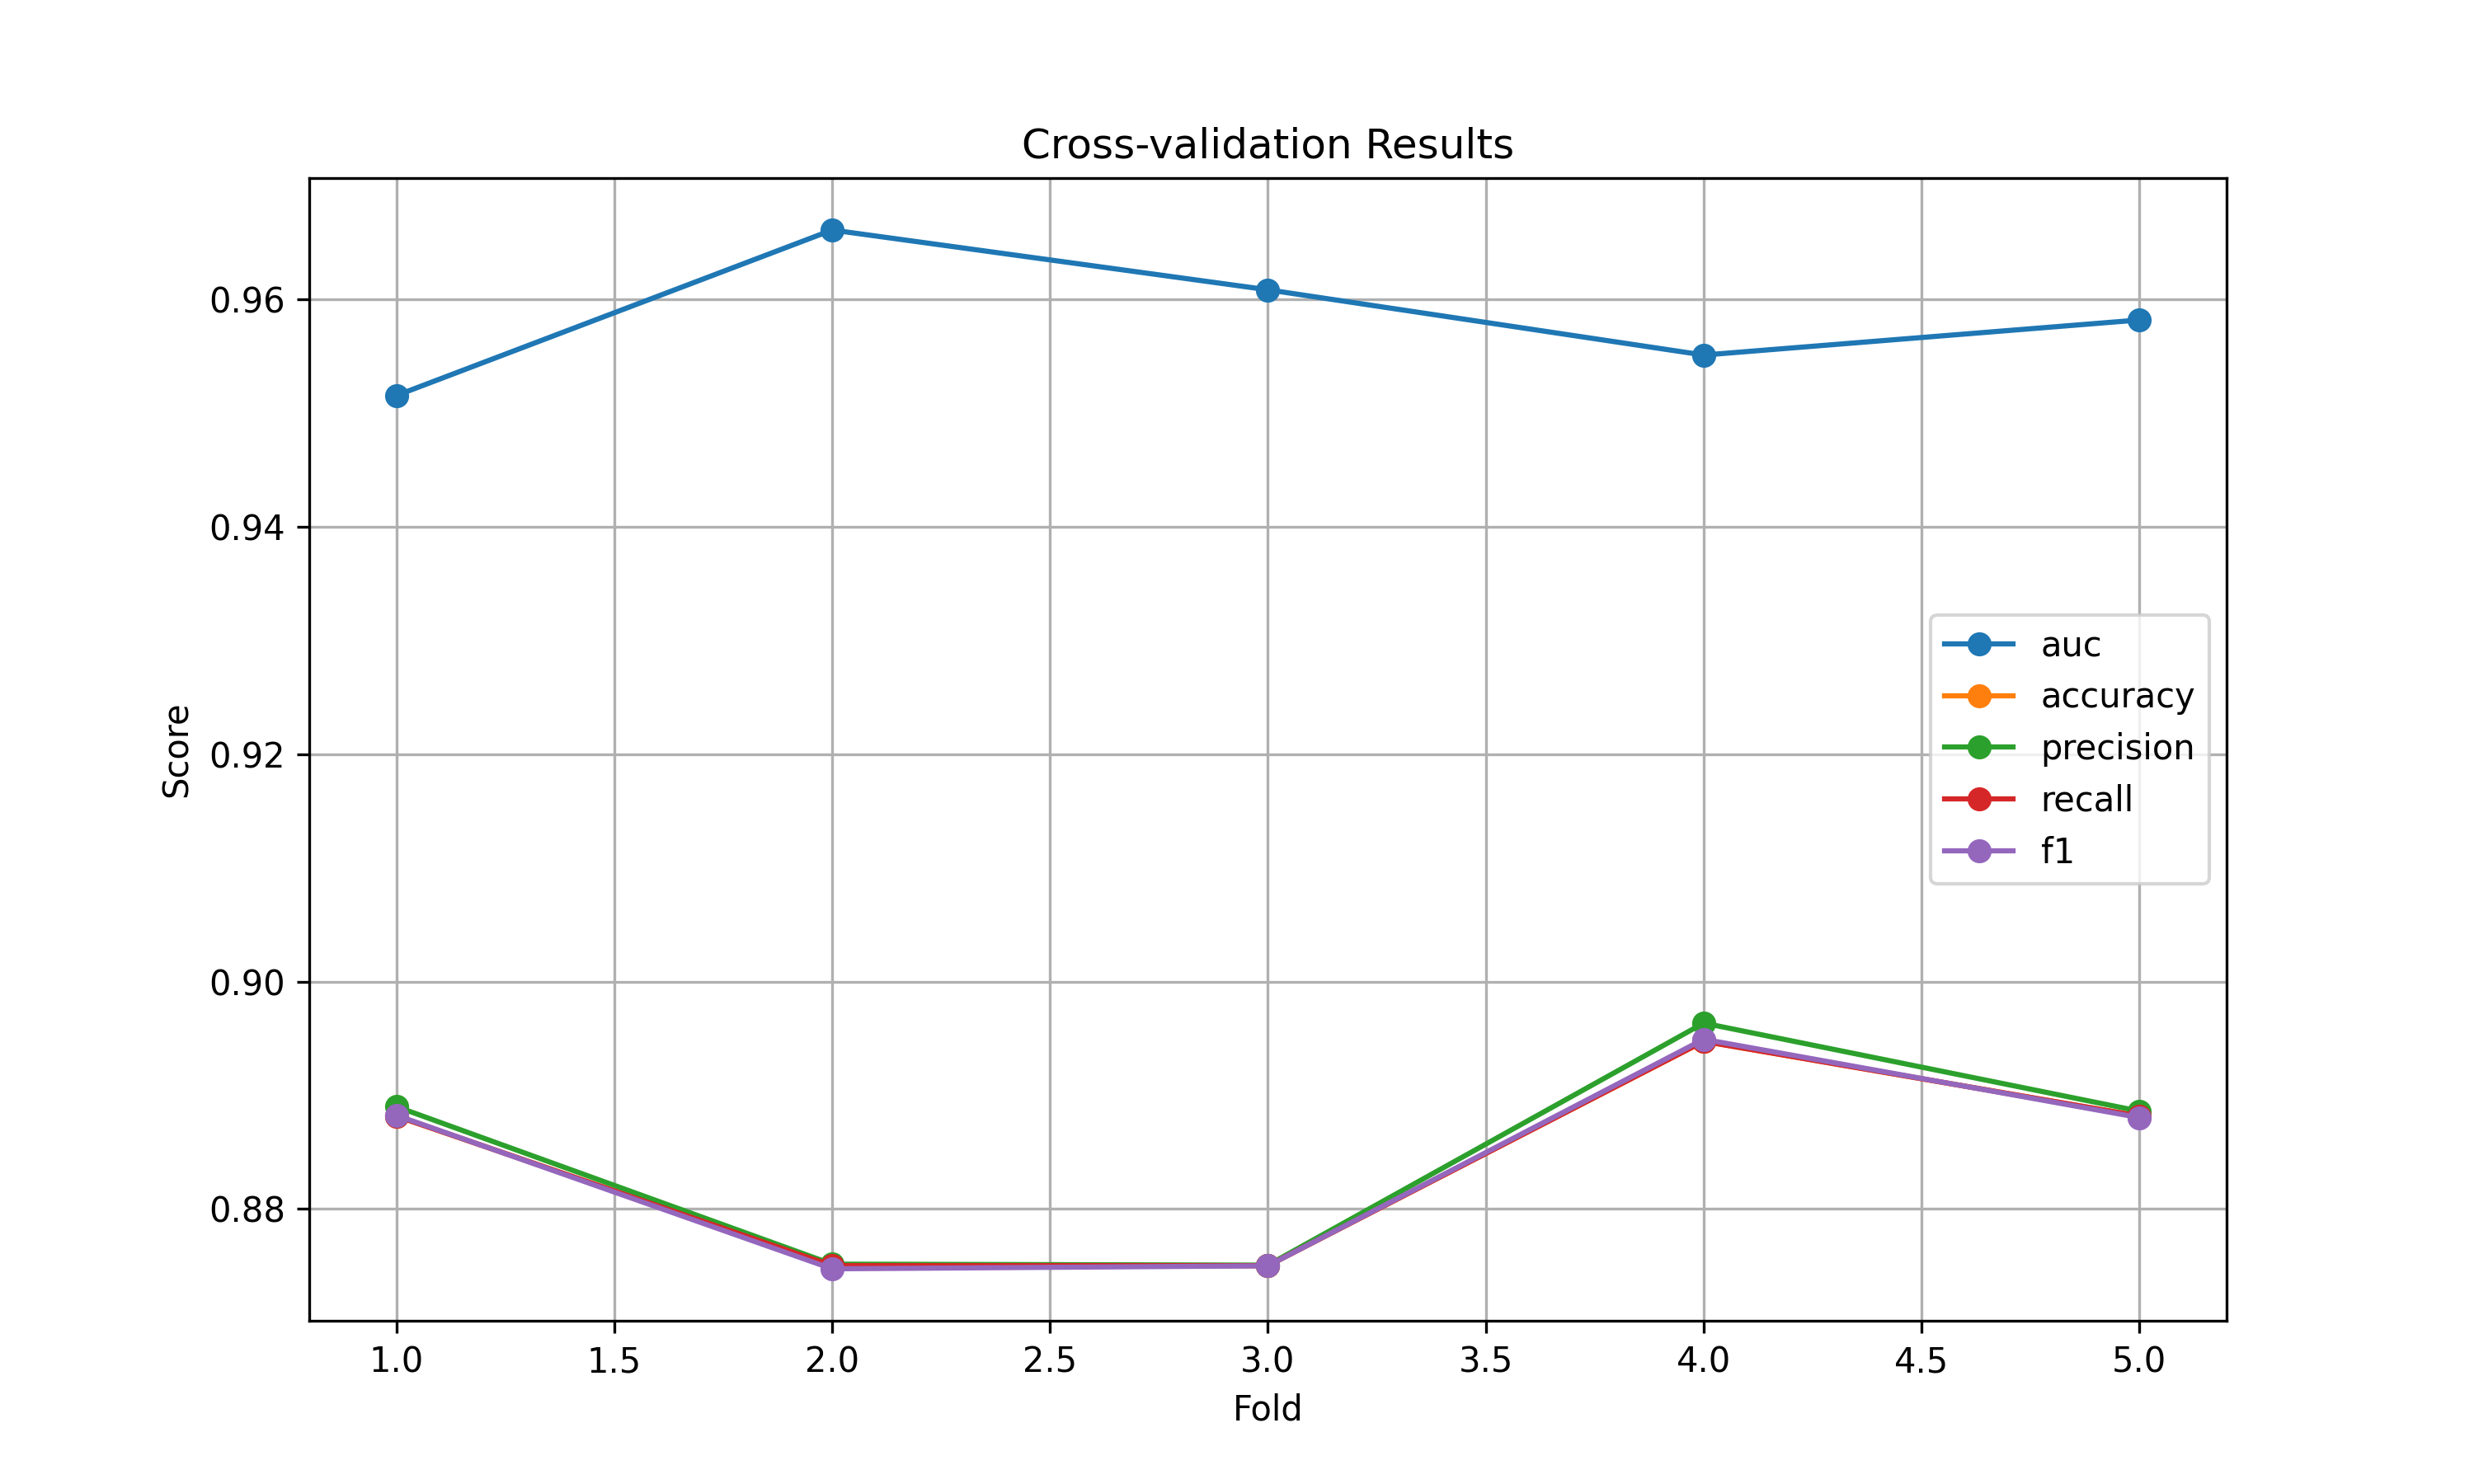
\includegraphics[width=0.9\textwidth]{images/neural_net_cv_results.png}
    \caption{نتایج کراس‌ولیدیشن ۵-فولدی مدل شبکه‌ی عصبی}
    \label{fig:neural_net_cv}
\end{figure}

در ادامه، برخی از نمودارهای ترسیم‌شده شامل توزیع کلاس‌ها (\lr{class distribution})، همبستگی ویژگی‌ها (\lr{feature correlations})، توزیع ویژگی‌ها برحسب کلاس (\lr{feature distribution by class})، منحنی \lr{ROC}، منحنی \lr{Precision-Recall}، ماتریس سردرگمی و مقایسه‌ی دقت مدل‌ها در سناریوهای مختلف نیز ارائه و تحلیل خواهند شد.

\begin{figure}
    \centering
    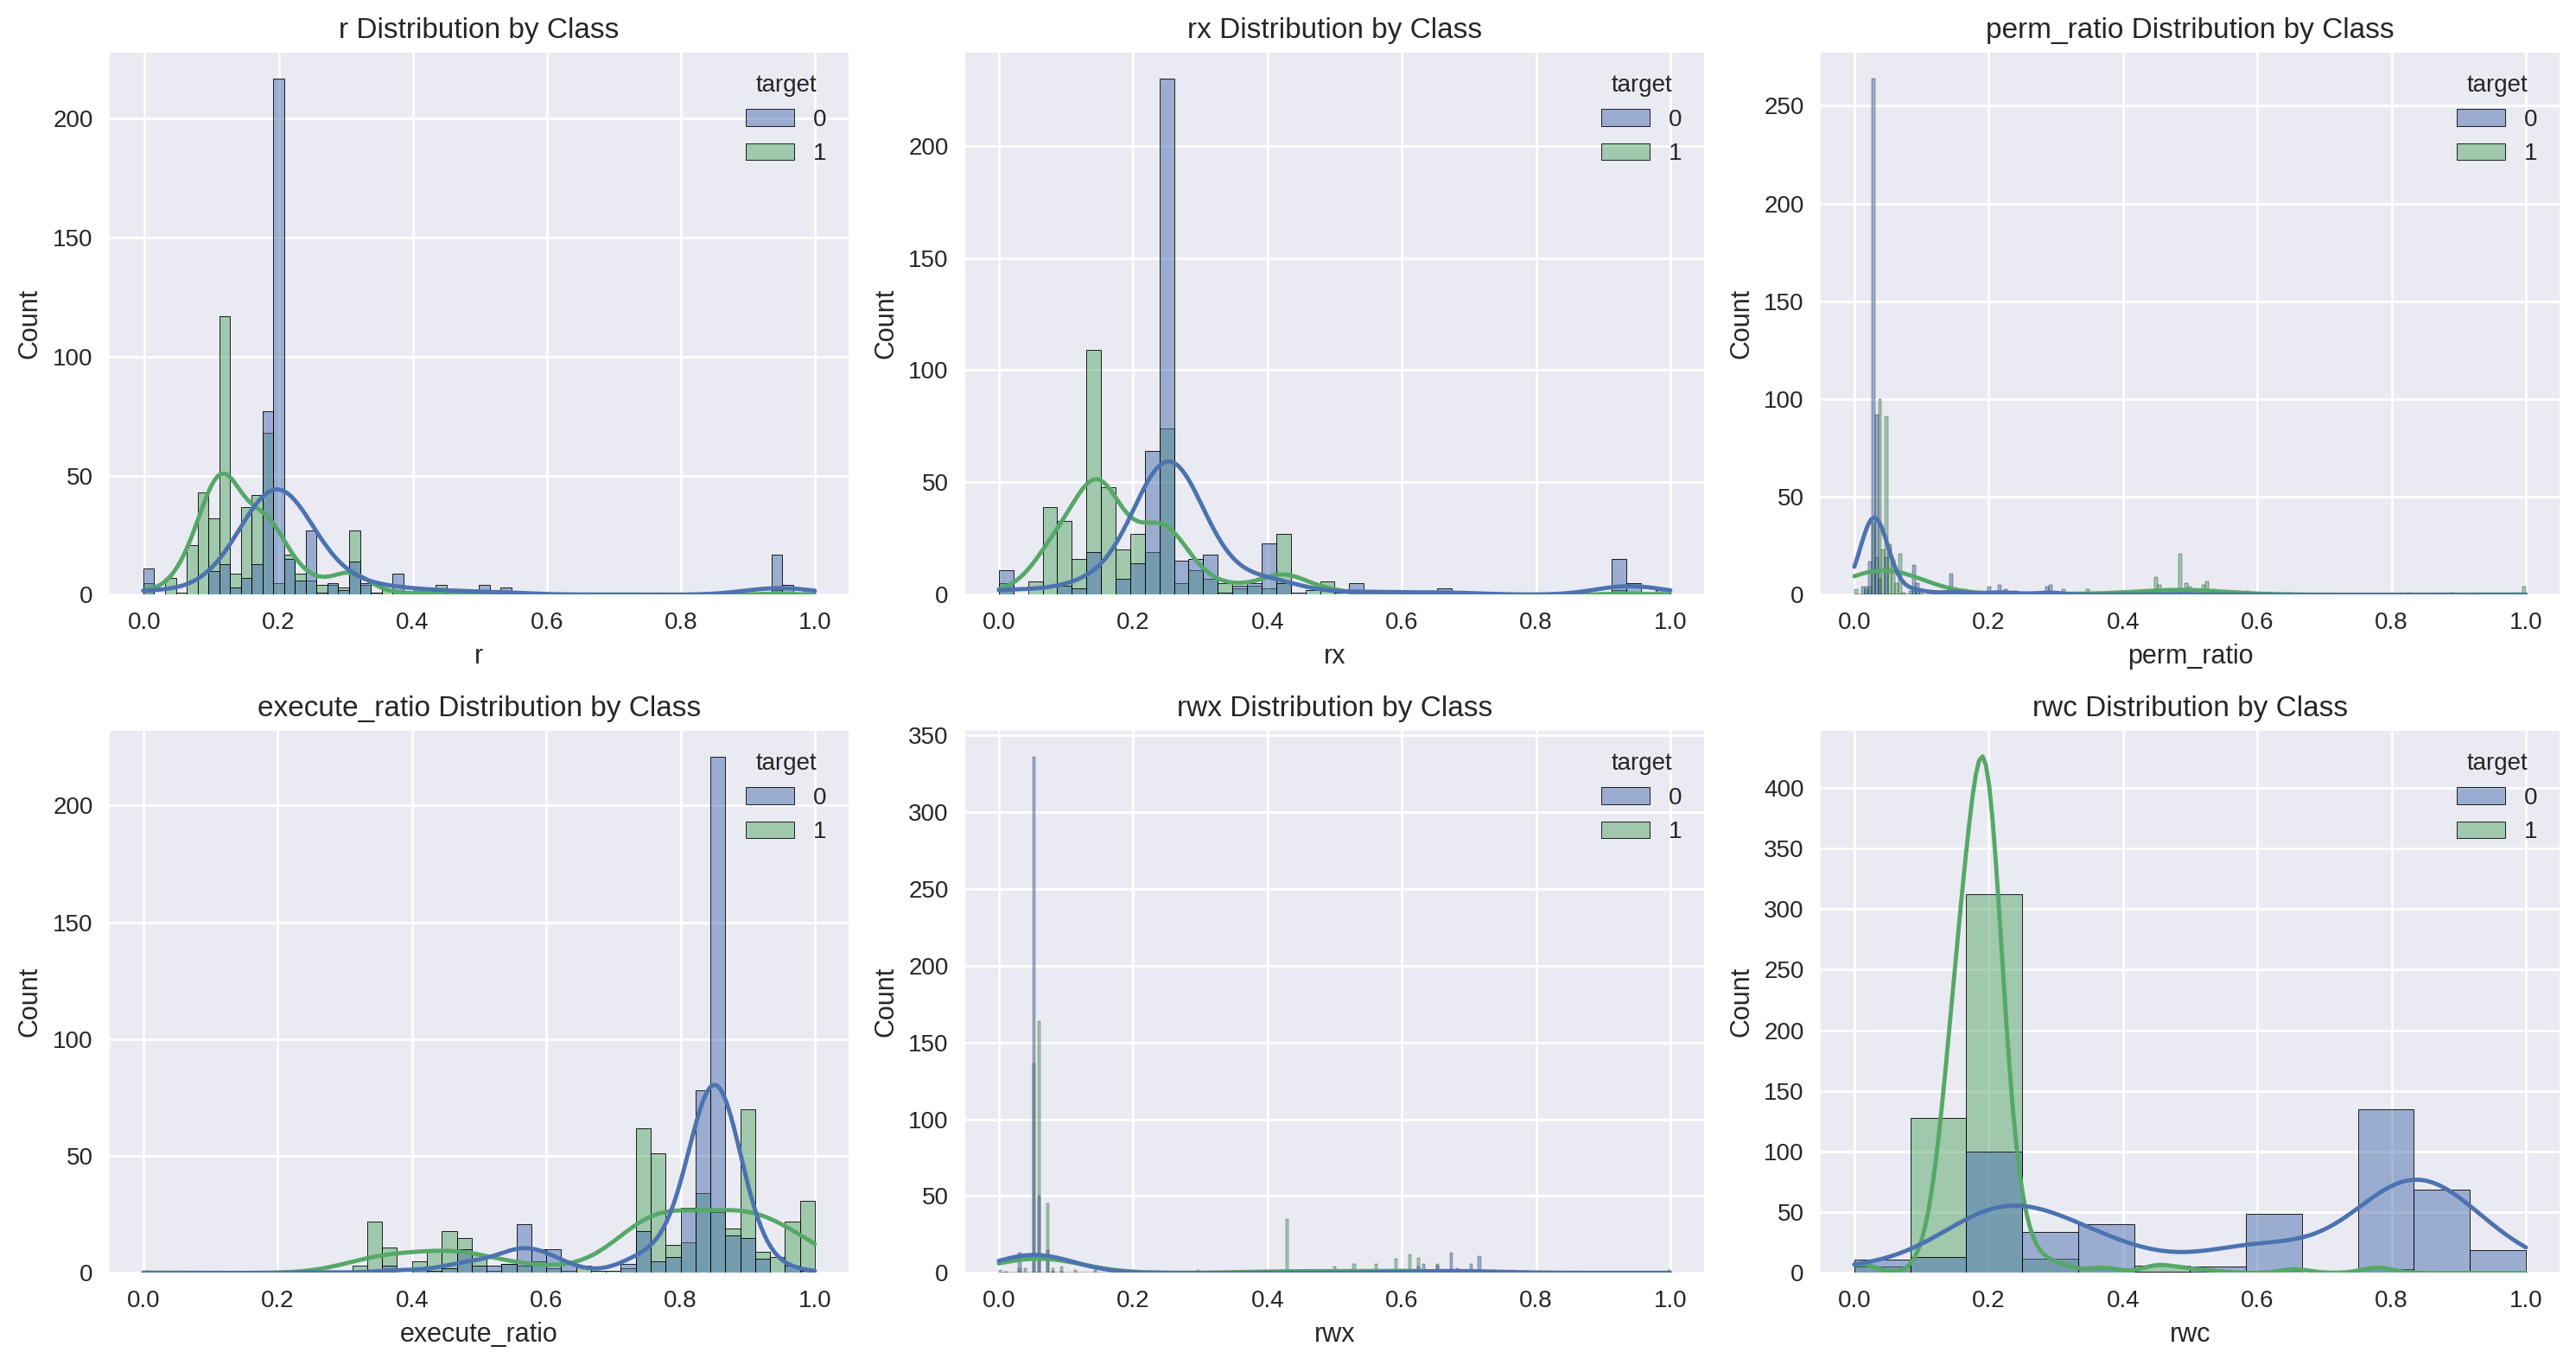
\includegraphics[width=0.85\textwidth]{images/top_feature_distributions.png}
    \caption{توزیع ویژگی‌های اصلی بر حسب کلاس (سالم/باج‌افزار)}
    \label{fig:class_dist}
\end{figure}

\begin{figure}
    \centering
    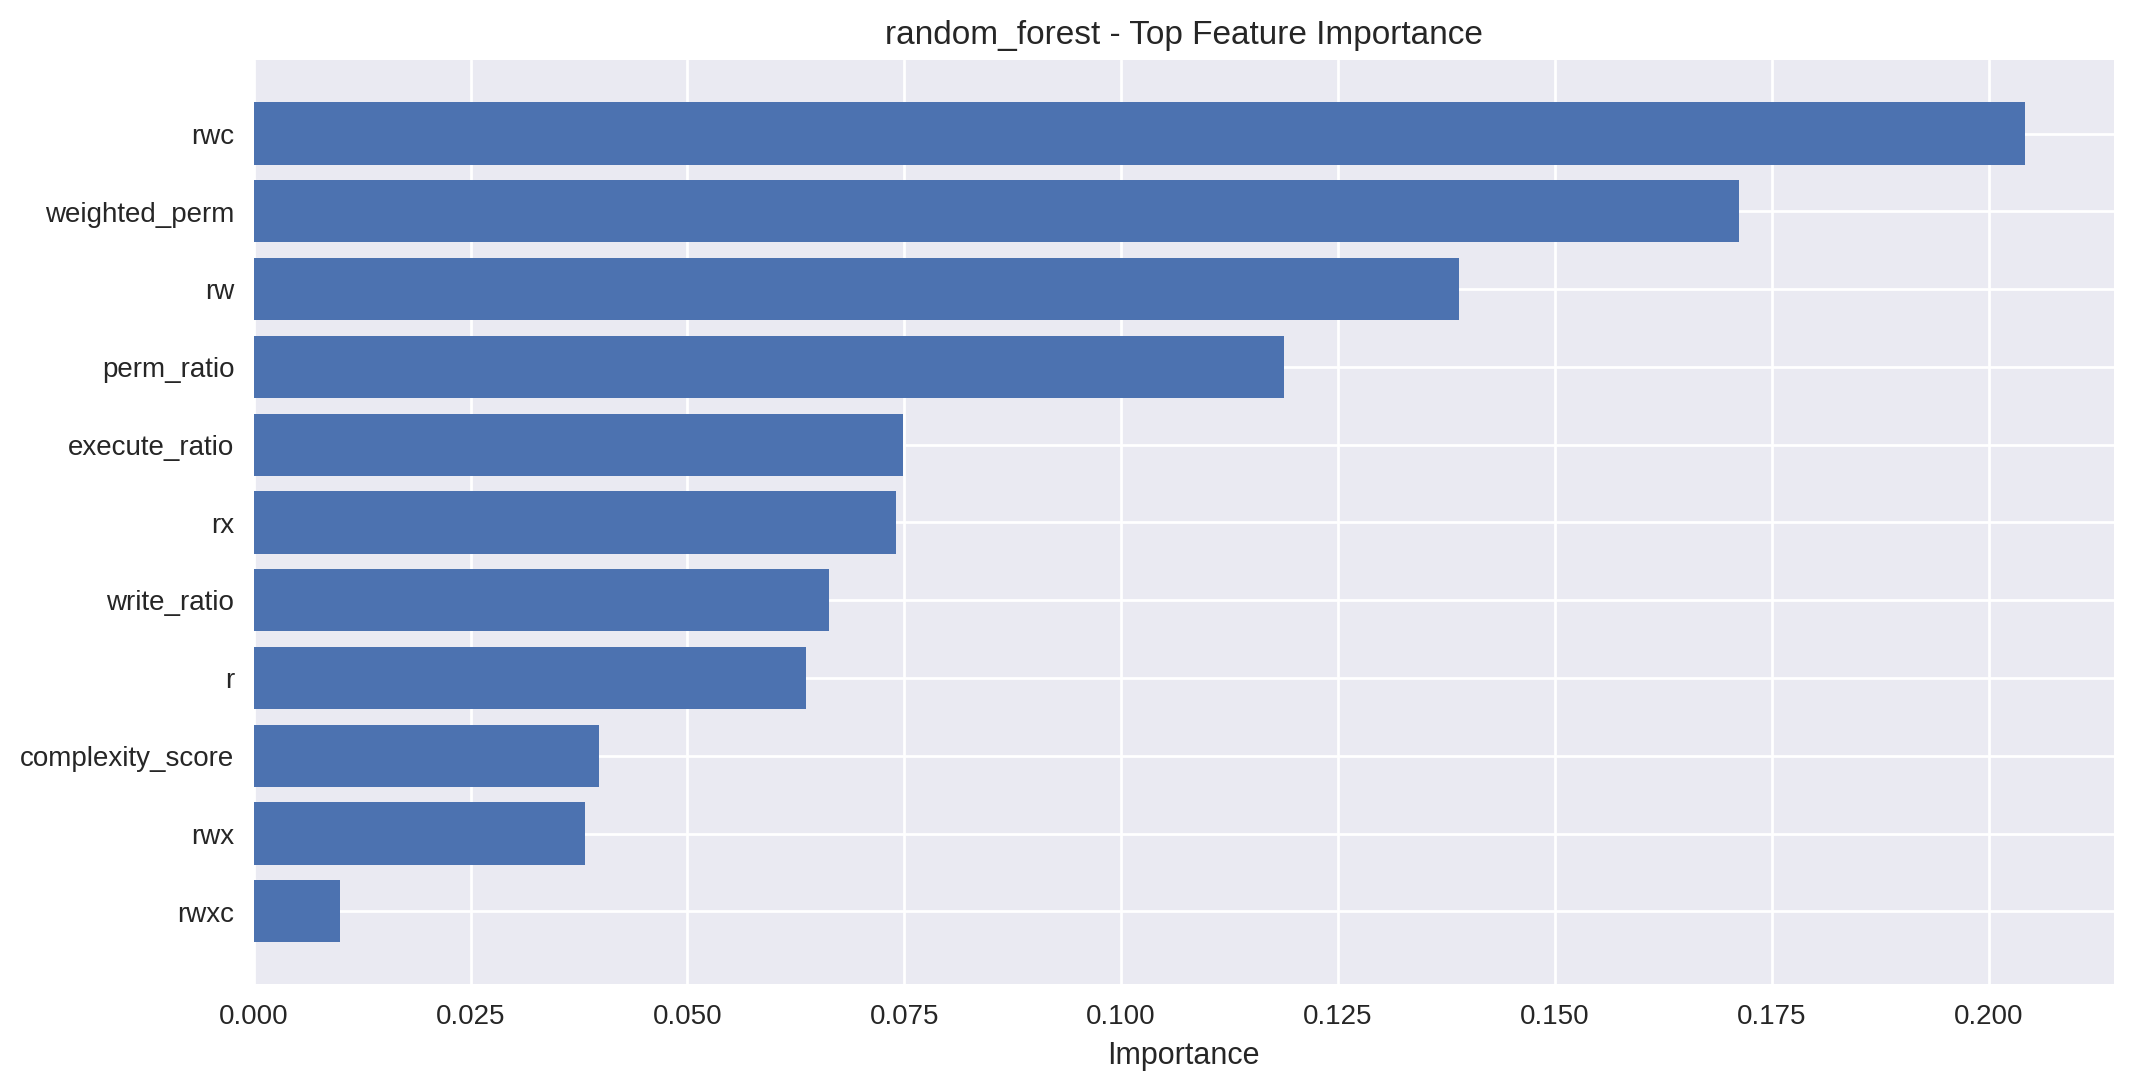
\includegraphics[width=0.85\textwidth]{images/random_forest_feature_importance.png}
    \caption{اهمیت ویژگی‌ها در مدل \lr{Random Forest}}
    \label{fig:feature_importance}
\end{figure}


\section{تحلیل مقایسه‌ای}


\subsection{منحنی ROC و ماتریس درهم‌ریختگی}
\begin{figure}[h]
    \centering
    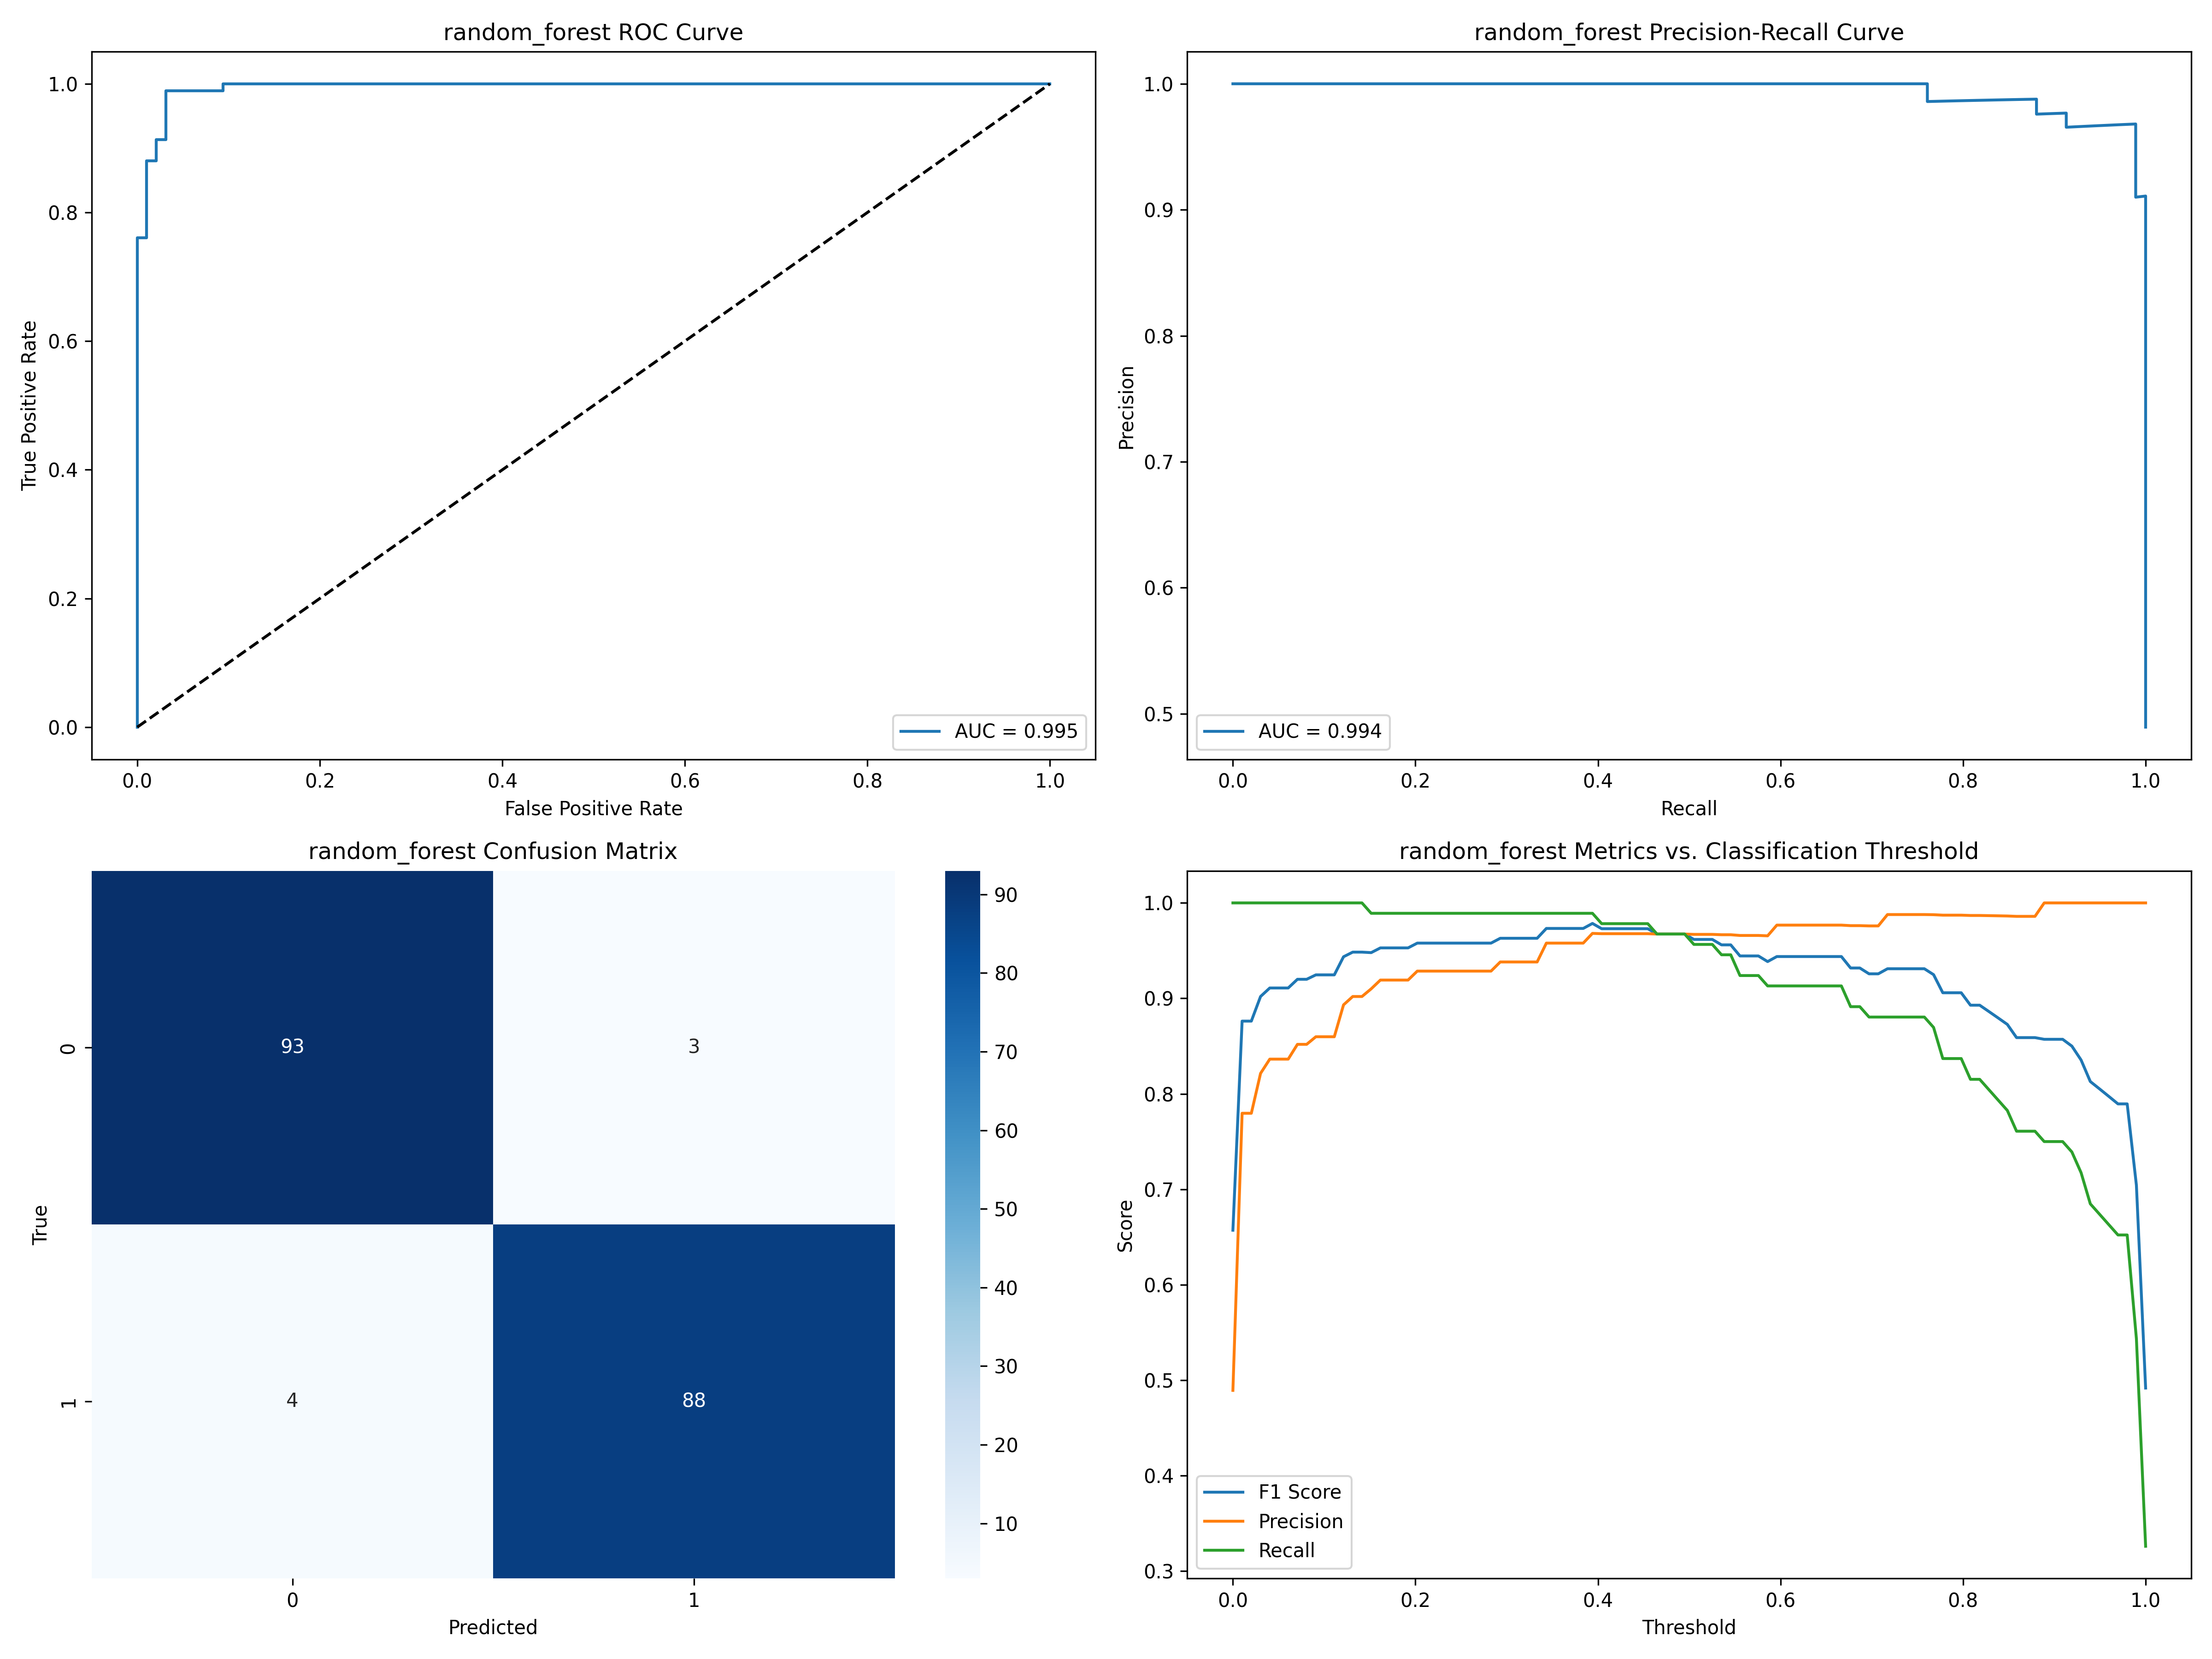
\includegraphics[width=0.6\textwidth]{images/random_forest_plots.png}
    \caption{منحنی ROC مدل‌ها با مساحت زیر منحنی (AUC). ماتریس درهم‌ریختگی مدل رندوم فارست (بهترین عملکرد)}
    \label{fig:conf_matـroc}
\end{figure}

\section{بحث و تحلیل}
\subsection{عملکرد MLP}
با وجود AUC بالا (۰.۹۵)، دقت پایین MLP (۰.۸۹) ناشی از:
\begin{itemize}
    \item تعداد محدود نمونه‌های آموزشی برای معماری عمیق
    \item نیاز به تنظیم دقیق نرخ یادگیری
    \item حساسیت به نویز در ویژگی‌های مهندسی‌شده
\end{itemize}

\subsection{مقایسه با RDPM}
\begin{table}[h]
    \centering
    \begin{tabular}{|l|c|c|}
        \hline
        \textbf{معیار} & \textbf{این پژوهش} & \textbf{RDPM} \\ \hline
        دقت & ۰.۹۲ & ۰.۸۷ \\ \hline
        Recall & ۰.۹۵ & ۰.۸۲ \\ \hline
        زمان اجرا (ms) & ۱۲ & ۲۵ \\ \hline
    \end{tabular}
    \caption{مقایسه با سیستم پایه RDPM}
\end{table}